%Je nach dem in welcher Sprache ihr euer Paper schreiben wollt,
%benutzt bitte entweder den Deutschen-Titel oder den Englischen (einfach aus- bzw. einkommentieren mittels '%')

%Deutsch
%\section{Methodischer Ansatz}

%Englisch
\section{Methodological Approach}
\label{methodology:methodological-approach}
This section outlines the methodological approach taken to design, implement, and evaluate an energy-aware server management solution for small and medium-sized enterprises (SMEs).
It describes the overall use case, the technical architecture of the prototype, and the integration of real-time energy consumption and electricity price data.

\subsection{Use Case Description}
\label{methodology:use-case-description}
The use case centers on an SME operating on-premise server infrastructure, seeking to optimize energy consumption and costs amid rising electricity prices. Key stakeholders include the SME IT administrator, who manages server operations and energy monitoring, and external data providers such as smart meters and electricity market APIs. The system aims to enable the administrator to schedule energy-intensive tasks during periods of lower electricity prices, thereby minimizing costs and supporting sustainability goals.
\begin{figure}[h!]
\centering
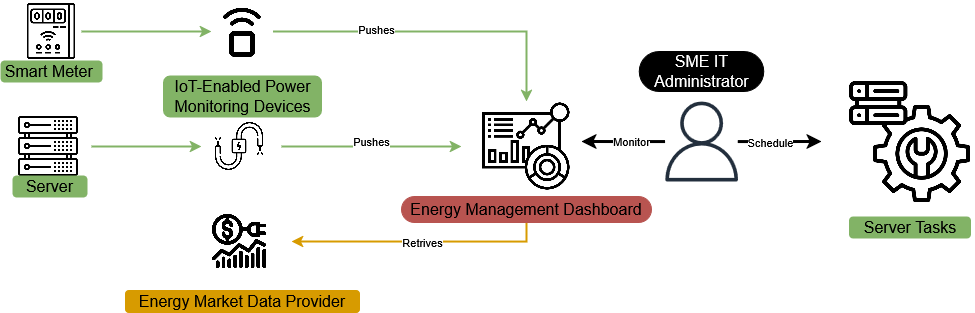
\includegraphics[width=0.8\textwidth]{fig/high_level_use_case.png}
\caption{Overall use case of server administrator utilizing the energy management dashboard.}
\label{fig:highleveluse}
\end{figure}
As illustrated in Figure~\ref{fig:highleveluse}, energy consumption data is continuously collected from both facility-level smart meters and device-level IoT power monitors. Simultaneously, real-time electricity prices are retrieved from market data providers (e.g., EPEX Spot). These data streams are integrated and visualized via a cloud-based dashboard, providing actionable insights and recommendations for workload scheduling.
\newpage
\subsection{Prototype}
\label{methodology:prototype}
The prototype implements a cloud-native architecture leveraging Amazon Web Services (AWS) to ensure scalability, reliability, and cost-effectiveness—key considerations for SMEs with limited IT resources. Figure~\ref{fig:architecture} illustrates the system architecture. The complete implementation details, including infrastructure as code and configuration files, are available in the project materials and are further described in Appendix~\ref{appendix:github-docs}.
\begin{figure}[htbp]
\centering
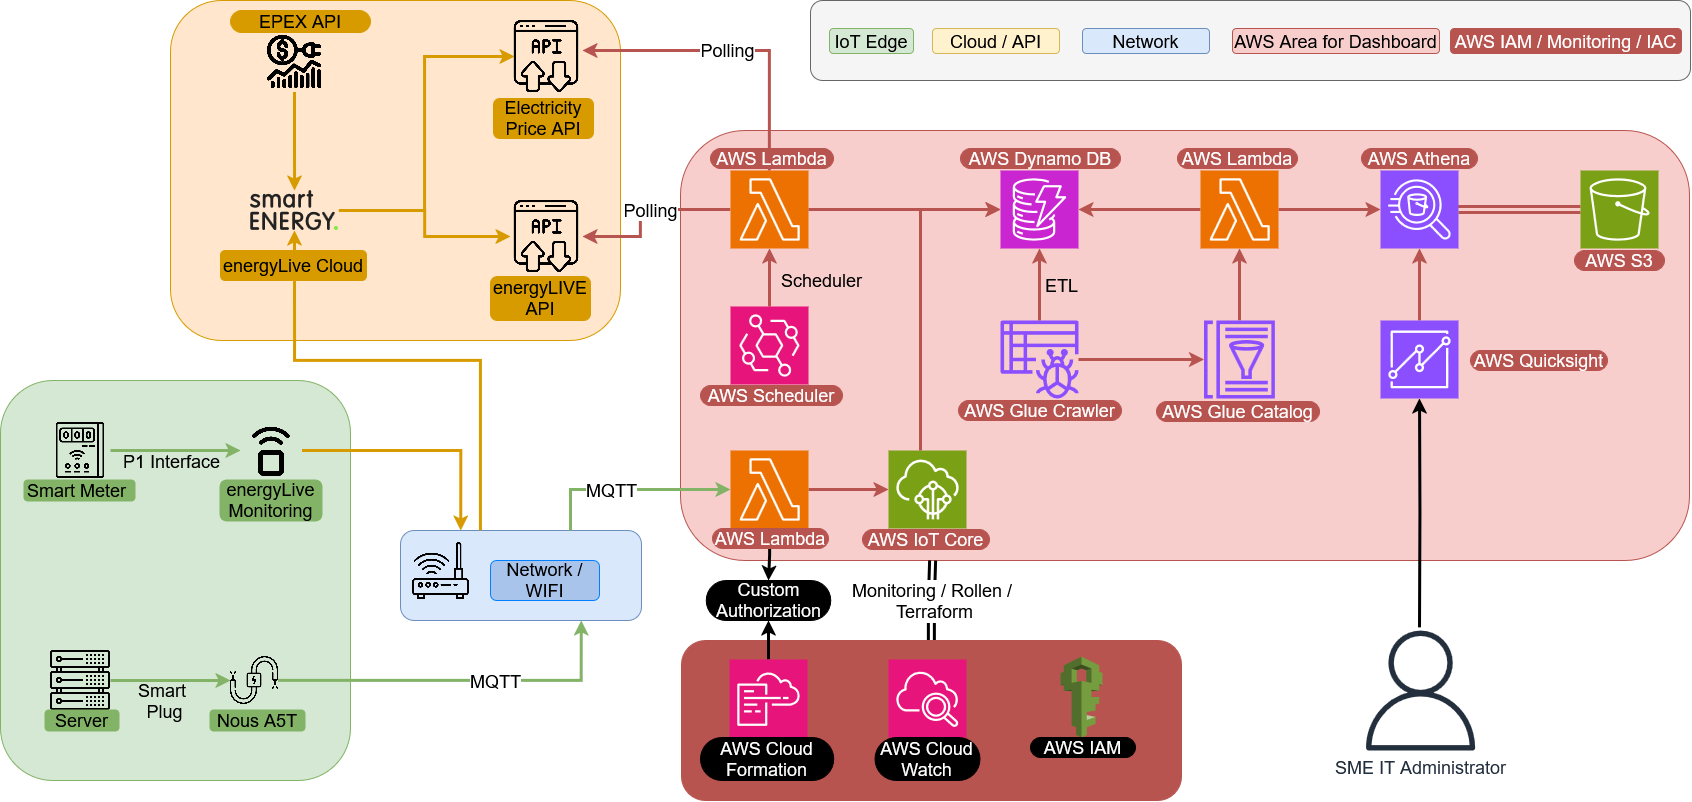
\includegraphics[width=1.1\textwidth]{fig/architektur_new_2.png}
\caption{System Architecture of the AWS implementation.}
\label{fig:architecture}
\end{figure}
At the edge, a smart meter with a P1 interface and a NOUS A5T smart plug\footnote{See Appendix~\ref{appendix:tasmota-config} for configuration details.} are deployed within the SME's local network. The smart meter provides aggregate facility-level data, while the NOUS A5T delivers device-specific power usage via MQTT. Data is ingested into the cloud using a hybrid of polling (for smart meter and market prices) and message-based (for IoT devices) mechanisms.
AWS Lambda functions, triggered by scheduled polling or MQTT messages, process incoming data. AWS IoT Core manages secure MQTT communication, while API Gateway and Lambda handle RESTful interactions with external APIs. All data is stored in AWS DynamoDB for low-latency access. AWS Glue and Athena enable automated data cataloging and ad hoc querying, respectively. Visualization is provided through AWS QuickSight dashboards, allowing administrators to correlate energy usage with market prices and identify optimization opportunities. Infrastructure is provisioned using AWS CloudFormation for reproducibility, and security is enforced via AWS IAM and CloudWatch.
\subsection{Evaluation Approach}
\label{methodology:evaluation-approach}
To evaluate the effectiveness of the approach, a comprehensive evaluation strategy is implemented that addresses technical performance, server energy consumption patterns, and economic impacts. This multi-faceted evaluation provides insights into both the system's technical capabilities and its practical utility for SME operators. The results of these experiments are presented in Section~\ref{results:results}.

Server energy consumption analysis forms the core of the measurement approach. Using the NOUS A5T PowerCable device, detailed measurements of a single server under various operational scenarios are conducted to establish energy consumption profiles. Specifically, the following workloads (WL) are examined:

\begin{enumerate}[label=WL\arabic*]
    \item \textbf{Maximum computational load:} Simulation of 100\% CPU utilization across all
    cores using the stress-ng tool on a Linux virtual machine. The stress-ng
    command will be configured to spawn CPU-intensive worker processes equal to
    the number of available virtual CPUs, ensuring maximum load across all cores.
    This scenario represents peak computational demand typical of batch processing
    or intensive data analysis tasks. \cite{stressng2020}

    \item \textbf{I/O stress testing:} This WL conduct I/O stress testing to evaluate
    power consumption during intensive disk operations. Using fio (Flexible I/O Tester),
    we will simulate maximum Solid State Drive (SSD) utilization with sequential and random read/write
    patterns. This I/O-intensive scenario represents workloads common in database operations,
    log processing, and large file transfers, providing insights into storage
    subsystem energy requirements under heavy load.

    \item \textbf{System reboot cycle:} Measurement of the overall power consumption profile
    during a full reboot sequence of the host machine, capturing the energy
    requirements during shutdown, boot, and system initialization phases. This
    provides insights into the energy costs associated with maintenance operations
    and system updates.

    \item \textbf{Maintenance operations:} Monitoring of energy consumption during typical
    maintenance activities, specifically the patching process of a Linux virtual
    machine. This scenario represents regular administrative tasks that SMEs must
    perform to maintain security and system integrity.

    \item \textbf{Idle state:} Establishing the baseline energy consumption when the server is
    in an idle state with minimal active processes. This measurement is crucial
    for understanding the fixed energy costs of maintaining server availability
    even during periods of low utilization. \cite{moran2024dissecting,agilewatts2022}
\end{enumerate}

For each WL, the total energy usage consumption is measured in kilowatt-hours (kWh) and power consumption patterns over time, establishing detailed energy profiles that can be correlated with specific operational states. These measurements reveal the energy intensity of different server activities and identify potential optimization opportunities, such as scheduling high-consumption tasks during periods of lower electricity pricing or implementing more efficient idle-state management.

To ensure reliable and representative measurements, each test scenario will be
conducted with specific time windows (TW):

\begin{enumerate}[label=TW\arabic*]
    \item For maximum computational load and I/O stress testing scenarios, each
    test window will span 15 minutes of load and 15 minutes of idle to capture steady-state 
    behavior and account for any thermal effects or performance throttling that may occur during
    sustained high-load operations.

    \item System reboot cycle measurements will be conducted over multiple
    iterations, with each complete cycle (shutdown to fully operational)
    typically lasting 5-10 minutes.

    \item Maintenance operation measurements will cover the entire duration of
    typical update processes, estimated at 5-10 minutes per session, including
    download, installation, and post-update system stabilization periods.

    \item Idle state measurements will be conducted over longer 60-minute windows
    during off-peak hours to establish accurate baseline consumption patterns and
    capture any periodic background system activities.
\end{enumerate}

A minimum cool-down period of 10 minutes has to be assured between test iterations to 
ensure thermal conditions return to baseline.

\subsection{Test Infrastructure Setup}
\label{methodology:test-infrastructure-setup}

To conduct the stress testing scenarios described in WL1 and WL2, a dedicated test infrastructure 
in the form of a Ubuntu 24.04.2 LTS virtual machine was established within a Proxmox virtualization
environment.

\subsubsection{CPU Stress Testing Configuration}
\label{methodology:cpu-stress-testing-configuration}

For maximum computational load testing (WL1), a dedicated stress-ng scheduling 
script was developed to generate sustained CPU load across all available cores. 
The stress-ng tool was selected for its ability to create reproducible, 
high-intensity computational workloads suitable for energy consumption analysis.

The CPU stress testing implementation (see Appendix~\ref{appendix:github-docs} 
for implementation details) includes the following characteristics:
\begin{itemize}
    \item \textbf{Full CPU utilization:} Spawns worker processes equal to the 
    number of available virtual CPUs (56 logical processors)
    \item \textbf{Sustained load patterns:} Maintains 100\% CPU utilization 
    for the entire 15-minute test duration
    \item \textbf{Thermal consideration:} Includes cooling periods between test 
    cycles to prevent thermal throttling effects
    \item \textbf{Automated scheduling:} Uses the \texttt{at} command for 
    precise timing synchronization with energy measurement intervals
    \item \textbf{Comprehensive logging:} Records CPU utilization metrics and 
    timestamps for correlation with power consumption data
\end{itemize}

The stress-ng configuration utilizes the command 
\texttt{stress-ng --cpu 56 --timeout 900s} to ensure maximum computational 
load across all processor cores. This approach simulates intensive batch 
processing workloads typical in SME environments, such as data analysis, 
compilation tasks, or scientific computing operations.

Similar to the I/O stress testing, the CPU stress script supports configurable 
test cycles with alternating 15-minute stress periods and 15-minute idle 
periods, enabling direct comparison of energy consumption between high-load 
and baseline states. The automated cleanup and logging mechanisms ensure 
consistent test conditions and comprehensive data collection for subsequent 
analysis.

\subsubsection{Storage Configuration}
\label{methodology:storage-configuration}
The original virtual machine configuration had insufficient free disk space for intensive
I/O testing that requires substantial temporary file creation. To address this limitation, a
dedicated 50GB virtual disk was provisioned and attached to the test virtual machine as a
secondary storage device.

The additional disk was formatted with the ext4 filesystem providing 50GB of available space
exclusively for I/O testing operations. The disk was configured with I/O threading enabled in 
the Proxmox hypervisor to maximize I/O performance and ensure realistic energy consumption
measurements under high-load conditions.
This configuration ensures that:

\begin{itemize}
    \item I/O testing operations do not interfere with system operations on the primary disk
    \item Sufficient space is available for creating large test files (up to 32GB total)
    \item Test data can be isolated and cleaned up after each measurement cycle
    \item Storage performance characteristics can be measured independently
\end{itemize}


\subsubsection{Automated Test Scheduling}
\label{methodology:automated-test-scheduling}
To ensure precise timing alignment with the 15-minute measurement intervals of the energy
monitoring system, automated test scheduling scripts were developed using the \texttt{at}
command scheduler. The FIO stress testing implementation (see Appendix~\ref{appendix:github-docs} 
for implementation details) includes the following characteristics:


\begin{itemize}
    \item \textbf{Configurable test cycles:} Support for multiple 15-minute I/O stress periods
    followed by 15-minute idle periods
    \item \textbf{Maximum I/O load generation:} Utilizes 4 parallel FIO jobs with 32-depth I/O queues,
    mixed random read/write patterns (70\% read, 30\% write), and variable block sizes (4KB to 1MB)
    \item \textbf{Direct I/O operations:} Bypasses operating system caches to ensure actual disk I/O
    and realistic power consumption
    \item \textbf{Automatic cleanup:} Removes test files after each cycle to prevent disk space
    exhaustion
    \item \textbf{Comprehensive logging:} Records detailed performance metrics and timestamps
    for correlation with energy measurements
\end{itemize}

This automated approach ensures that I/O stress testing can be precisely 
synchronized with energy measurement intervals, enabling accurate correlation 
between storage workload intensity and power consumption patterns.